\chapter[Local Thorin Structure]{Local Thorin Structure: Ramanujan Bounds, Function Fields and Hitting Times}\label{ch:10c}

Ramanujan conjectured in 1916 that $|\tau(p)|\le2p^{11/2}$ \cite{ramanujan1916}. The bound concerns a single Euler factor: it says exactly that the two roots of $1-\tau(p)X+p^{11}X^2$ have the same absolute value. The Riemann hypothesis for $L(s,\Delta)$ is a statement about all Euler factors at once, and nothing in the classical theory makes the two look alike. Chapter~\ref{ch:10b} recast the generalized Riemann hypothesis for an automorphic $L$ function as a positivity property: the reciprocal of the completed function, evaluated at $\sqrt s$, is the Laplace transform of a generalized gamma convolution, with Thorin measure carried by the squared ordinates of the zeros. In this chapter we apply the same test to a single Euler factor and find that it is passed exactly when the Ramanujan bound holds. The slogan is that \emph{Ramanujan is local Thorin and Riemann is global Thorin}. We then follow the local Thorin measures in four directions: into the explicit formula, where they appear as damped periodic combs; into random Euler products with Sato Tate angles, where they become point processes; into function fields and regular graphs, where global Thorin is a theorem; and into hitting times of Hecke walks on trees and isogeny graphs, where Thorin measures are spectra and Keilson's theorem turns the Ramanujan bound into statements about passage times. The last section returns to the extreme value laws of Chapter~\ref{ch:11} and identifies their exponent measures.

Throughout, a GGC is as in Definition~\ref{def:ch10ggc}, we write $L=\log p$ (or $\log q$) when the prime is fixed, and $E,E_1,E_2,\dots$ are independent standard exponential variables.

\section{The local Thorin criterion}\index{local Thorin criterion}

Let $\pi$ be a cuspidal automorphic representation of $\GL_2(\A_\Q)$ with trivial central character, in the unitary normalisation, and let $p$ be a prime at which $\pi$ is unramified. Its Euler factor is
\[
L_p(s)=(1-\alpha p^{-s})^{-1}(1-\beta p^{-s})^{-1},\qquad \alpha\beta=1 .
\]
Unitarity of $\pi_p$ makes the Satake set $\{\alpha,\beta\}$ stable under $z\mapsto\bar z^{-1}$, so either $|\alpha|=1$ or $\alpha$ is real; in both cases $x_p=\alpha+\beta$ is real, and $|x_p|\le2$ exactly when $|\alpha|=1$. The Ramanujan Petersson conjecture at $p$ is the statement $|\alpha|=|\beta|=1$. We complete the local factor by the symmetrising factor $p^w$:
\[
E_p(w)=p^{w}L_p(w)^{-1}=p^w-x_p+p^{-w}=2\cosh(wL)-x_p,\qquad L=\log p .
\]
It is entire, even and real on the real axis, the exact local analogue of $\Xi_\pi$. Its zeros are the local zeros of $L_p(w)^{-1}$, and the Ramanujan bound says they lie on $\Re w=0$. So the local centre is $\Re w=0$, while the global centre in the same normalisation is $\Re s=\frac12$; Section~\ref{sec:10ccombs} measures the difference.

\begin{lemma}\label{lem:10cproduct}
For $0<\theta\le\pi$ and all $w\in\C$,
\[
\cosh w-\cos\theta=(1-\cos\theta)\prod_{k\in\Z}\Bigl(1+\frac{w^2}{(\theta+2\pi k)^2}\Bigr),
\]
the product converging absolutely and locally uniformly.
\end{lemma}

\begin{proof}
The left side is even and entire, so it equals $G(w^2)$ with $G(u)=\sum_{n\ge0}u^n/(2n)!-\cos\theta$ entire. Since $|G(u)|\le\cosh|u|^{1/2}+1$, $G$ has order at most $\frac12$. Its zeros are the values $u=w^2$ with $\cosh w=\cos\theta$, that is $w=\pm i(\theta+2\pi k)$, so $u_k=-(\theta+2\pi k)^2$, $k\in\Z$. If $0<\theta<\pi$ the $u_k$ are distinct simple zeros, because $G'(u_k)=\sinh(w)/(2w)$ with $\sinh w=\pm i\sin\theta\ne0$. If $\theta=\pi$ then $u_k=u_{-k-1}$, and both sides acquire double zeros, since $\cosh w+1=2\cosh^2(w/2)$; listing $u_k$ over $k\in\Z$ counts this multiplicity correctly. As $\sum_k|u_k|^{-1}<\infty$ and $G$ has order less than one, Hadamard's theorem gives $G(u)=G(0)\prod_k(1-u/u_k)$ with no exponential factor, and $G(0)=1-\cos\theta\ne0$.
\end{proof}

The main result of this section needs a classical fact about Laplace transforms of positive measures, due in the setting of Dirichlet series to Landau \cite{landau1905} and going back to Pringsheim's theorem on power series; see Widder \cite{widder1941}.

\begin{lemma}[Pringsheim and Landau]\label{lem:10clandau}
Let $\mu$ be a positive measure on $[0,\infty)$ whose Laplace transform $\varphi(s)=\int e^{-sx}\mu(dx)$ converges for $s>\sigma_c$ and diverges for $s<\sigma_c$, where $-\infty<\sigma_c<\infty$. Then $\varphi$ has no analytic continuation to a neighbourhood of $\sigma_c$.
\end{lemma}

\begin{proof}
The proof of Lemma~\ref{lem:ch09landau} applies verbatim to $\mu$, since it uses only the positivity of the measure $\sum_na_n\delta_{\log n}$.
\end{proof}

\begin{theorem}[Local Thorin criterion, this book]\label{thm:10clocal}\index{Thorin comb}
Let $L>0$ and $x\in\R$, and put
\[
f_x(s)=\frac{2-x}{2\cosh(L\sqrt s)-x},\qquad s>0 .
\]
Then $f_x$ is the Laplace transform of a probability law on $[0,\infty)$ if and only if $-2\le x<2$. In that case, writing $x=2\cos\theta$ with $0<\theta\le\pi$, the law is a GGC with drift $0$ and Thorin measure
\[
\tau_{\theta,L}=\sum_{k\in\Z}\delta_{t_k},\qquad t_k=\Bigl(\frac{\theta+2\pi k}{L}\Bigr)^2,
\]
namely the law of $\sum_{k\in\Z}E_k/t_k$, with mean $L^2/(2-x)$.
\end{theorem}

\begin{proof}
Suppose $-2\le x<2$. By Lemma~\ref{lem:10cproduct} with $w=L\sqrt s$, $f_x(s)=\prod_k(1+s/t_k)^{-1}$ with all $t_k>0$, so Theorem~\ref{thm:10babstract}, (a) implies (c), applied to $z\mapsto(2\cosh(Lz)-x)/(2-x)$, shows that $f_x$ is the Laplace transform of the GGC $\sum_kE_k/t_k$ with Thorin measure $\sum_k\delta_{t_k}$. Comparing the coefficients of $w^2$ in the lemma gives its mean $\sum_kt_k^{-1}=L^2/(4\sin^2(\theta/2))=L^2/(2-x)$.

Suppose $x>2$ and write $x=2\cosh a$ with $a>0$. Then $s\mapsto2\cosh(L\sqrt s)-x$ increases on $[0,\infty)$ from $2-x<0$ and vanishes at $s_0=(a/L)^2$, so $f_x(s)>1$ on $(0,s_0)$ and $f_x(s)\to+\infty$ as $s\uparrow s_0$. A Laplace transform of a probability law is bounded by $1$ on $(0,\infty)$, so $f_x$ is not one.

Suppose $x<-2$ and write $x=-2\cosh a$ with $a>0$. Since $\cosh(L\sqrt s)$ is an entire function of $s$, $f_x$ is meromorphic on $\C$, with poles where $\cosh(L\sqrt s)=-\cosh a$, that is at $s=\bigl((a+i(2k+1)\pi)/L\bigr)^2$, $k\in\Z$. These poles are not real, since $a\ne0$ and $(2k+1)\pi\ne0$. On the real axis $f_x$ is finite: for $s\ge0$ the denominator is at least $2+2\cosh a$, and for $s=-u^2<0$ it equals $2\cos(Lu)+2\cosh a>0$. Suppose $f_x(s)=\int e^{-sy}\mu(dy)$ for $s>0$ with $\mu$ a probability. Let $\sigma_c\le0$ be the abscissa of convergence. The Laplace integral is holomorphic on $\Re s>\sigma_c$ and agrees with $f_x$ on $(0,\infty)$, so by uniqueness of continuation it agrees with $f_x$ on the real interval $(\sigma_c,\infty)$. If $\sigma_c>-\infty$ then $f_x$ continues it analytically to a neighbourhood of $\sigma_c$, contradicting Lemma~\ref{lem:10clandau}. So $\sigma_c=-\infty$, the integral converges absolutely on $\C$ and defines an entire function equal to $f_x$, which is impossible because $f_x$ has poles. Finally $x=2$ makes the numerator vanish.
\end{proof}

The proof shows that for a single Euler factor the GGC property is automatic once $f_x$ is a Laplace transform at all: positivity alone forces the Thorin structure. The atoms $t_k$ are the squares of the ordinates $(\theta+2\pi k)/L$ of the local zeros $w=\pm i(\theta+2\pi k)/L$ of $E_p$, exactly as the global Thorin atoms of Chapter~\ref{ch:10b} are the squares $\gamma_k^2$. We call $\tau_{\theta,L}$ the \emph{local Thorin comb}; on the ordinate axis it consists of the two arithmetic progressions $(\pm\theta+2\pi\Z)/L$.

\begin{corollary}[this book]\label{cor:10cramanujan}\index{Ramanujan Petersson conjecture}
Let $\pi$ be as above and $p$ unramified with $x_p\ne2$. The Ramanujan Petersson conjecture holds at $p$ if and only if $s\mapsto E_p(0)/E_p(\sqrt s)$ is the Laplace transform of a probability law on $[0,\infty)$, and then this law is a GGC with Thorin measure $\tau_{\theta_p,\log p}$, $x_p=2\cos\theta_p$.
\end{corollary}

\begin{proof}
$E_p(0)/E_p(\sqrt s)=f_{x_p}(s)$ with $L=\log p$, and $|\alpha|=1$ if and only if $-2\le x_p\le2$.
\end{proof}

The excluded value $x_p=2$ ($\alpha=\beta=1$) is tempered, and there $E_p$ has a double zero at $w=0$: then $1/E_p(\sqrt s)=(L^2s)^{-1}\prod_{k\ne0}(1+sL^2/(2\pi k)^2)^{-1}$, and, as in the rank discussion of Chapter~\ref{ch:10}, the factor $(L^2s)^{-1}$ is a degenerate Thorin atom of mass $1$ at the origin (Exercise~\ref{ex:10cdegenerate}).

\begin{example}[The discriminant form]
For $\pi$ attached to $\Delta$, $x_p=\tau(p)p^{-11/2}$. Deligne's theorem \cite{deligne1974}, the Ramanujan conjecture for $\Delta$, gives $|x_p|\le2$, and $x_p\ne\pm2$ since $p^{11/2}$ is irrational. So local Thorin holds at every prime, and by Corollary~\ref{cor:10cramanujan} this statement is equivalent to the Ramanujan conjecture for $\Delta$. Global Thorin for $\Delta$, by Theorem~\ref{thm:ch10ggc} and Chapter~\ref{ch:10b}, is the Riemann hypothesis for $L(s,\Delta)$, which is open. At $p=2$, $x_2=-0.53033$, $\theta_2=1.83917$, and the first atoms of $\tau_{\theta_2,\log2}$ are $7.0403$ and $41.105$; the local law has mean $(\log2)^2/(2-x_2)=0.18988$.
\end{example}

The local criterion also grades failures of Ramanujan. Write $\alpha=e^{i(\varphi+i\eta)}$ with $\varphi,\eta$ real, so that $|\alpha|=e^{-\eta}$ and $x_p=2\cos(\varphi+i\eta)$. The zeros of $E_p$ are $w=i(\pm(\varphi+i\eta)+2\pi k)/L$, with real parts $\mp\eta/L$. For Maass forms on $\GL_2$ over $\Q$, Kim and Sarnak proved $|\alpha_p|\le p^{7/64}$ \cite{kimsarnak2003}, that is $|\eta|\le\frac{7}{64}\log p$, so every local zero lies in the strip $|\Re w|\le\frac{7}{64}$. Squaring, the poles $s=w^2$ of $s\mapsto1/E_p(\sqrt s)$ lie in the parabolic region $P_{7/64}=\{w^2:|\Re w|\le\frac7{64}\}$ of Chapter~\ref{ch:10b}. Thus, writing $\Theta^{(p)}_\sigma$ for the local parabolic condition that all poles of $1/E_p(\sqrt s)$ lie in $P_\sigma$, the Kim Sarnak theorem is $\Theta^{(p)}_{7/64}$ at every unramified $p$, and the Ramanujan conjecture is $\Theta^{(p)}_0$, the degenerate parabola $P_0=(-\infty,0]$, which by Theorem~\ref{thm:10clocal} is local Thorin. Globally, $\Theta_{1/2}$ holds for every $\pi$ (Chapter~\ref{ch:10b}), but $\Theta_\sigma$ with $\sigma<\frac12$, a zero free strip of positive width, is known for no automorphic $L$ function over $\Q$, while the local exponent $\frac{7}{64}$ is a theorem.

\section{Local combs and the explicit formula}\label{sec:10ccombs}\index{explicit formula}

For an even test function $h$ we define the \emph{comb sum} of $p$ as the sum of $h$ over the ordinates of the local zeros:
\[
c_p(h)=\sum_{k\in\Z}\Bigl[h\Bigl(\frac{\theta_p+2\pi k}{L}\Bigr)+h\Bigl(\frac{-\theta_p+2\pi k}{L}\Bigr)\Bigr],\qquad L=\log p .
\]

\begin{lemma}\label{lem:10cpoisson}
Let $h$ be an even Schwartz function and $H(x)=\int h(t)e^{-ixt}\,dt$. Then for every $\theta\in\R$ and $L>0$,
\[
\sum_{k\in\Z}\Bigl[h\Bigl(\frac{\theta+2\pi k}{L}\Bigr)+h\Bigl(\frac{-\theta+2\pi k}{L}\Bigr)\Bigr]=\frac{L}{\pi}H(0)+\frac{2L}{\pi}\sum_{m\ge1}\cos(m\theta)\,H(mL).
\]
\end{lemma}

\begin{proof}
Let $g(y)=h((\theta+2\pi y)/L)$, a Schwartz function. Poisson summation gives $\sum_kg(k)=\sum_m\hat g(m)$ with $\hat g(\xi)=\int g(y)e^{-2\pi i\xi y}dy$. Substituting $t=(\theta+2\pi y)/L$, so $2\pi y=Lt-\theta$,
\[
\hat g(m)=\frac{L}{2\pi}\int h(t)e^{-im(Lt-\theta)}dt=\frac{L}{2\pi}e^{im\theta}H(mL).
\]
The progression with $-\theta$ gives $\frac{L}{2\pi}\sum_me^{-im\theta}H(mL)$. Adding, and using that $H$ is even because $h$ is, the total is $\frac{L}{2\pi}\sum_{m\in\Z}2\cos(m\theta)H(mL)$, which is the stated formula after separating $m=0$ and pairing $\pm m$.
\end{proof}

So the comb of $p$ has mean density $L/\pi$ and oscillatory Fourier coefficients $\frac{2L}{\pi}\cos(m\theta_p)$ at the frequencies $m\log p$. Compare Weil's explicit formula \cite{weil1952}, which we state in the form of Iwaniec and Kowalski \cite{iwanieckowalski2004}, Chapter~5, for $\Delta$ in the unitary normalisation: $L(s,\Delta)=\sum\tau(n)n^{-11/2-s}$, $\Lambda(s,\Delta)=(2\pi)^{-s-11/2}\Gamma(s+\frac{11}{2})L(s,\Delta)$, nontrivial zeros $\frac12+i\gamma$ counted with multiplicity (the zeros $6+i\gamma$ of the classical normalisation of Chapter~\ref{ch:10}).

\begin{theorem}[Weil; see \cite{iwanieckowalski2004}]\label{thm:10cexplicit}
Let $h$ be even and holomorphic in $|\Im t|<\frac12+\varepsilon$, with $h(t)\ll(1+|t|)^{-1-\delta}$ there, and $H(x)=\int h(t)e^{-ixt}dt$. Then
\begin{multline*}
\sum_\gamma h(\gamma)=\frac{1}{2\pi}\int_{\R}h(t)\,2\Re\Bigl[-\log2\pi+\frac{\Gamma'}{\Gamma}(6+it)\Bigr]dt\\
-\frac1\pi\sum_p\sum_{m\ge1}2\cos(m\theta_p)\,\log p\;p^{-m/2}H(m\log p).
\end{multline*}
\end{theorem}

Here the number $(\alpha_p^m+\beta_p^m)\log p=2\cos(m\theta_p)\log p$ is the coefficient of $p^{-ms}$ in $-L'/L(s,\Delta)$. Lemma~\ref{lem:10cpoisson} now gives a term by term dictionary.

\begin{proposition}[this book]\label{prop:10cdictionary}
For every prime $p$ and every $h$ as in Theorem~\ref{thm:10cexplicit} that is also Schwartz on $\R$, the contribution of $p$ to the prime side of the explicit formula is obtained from the oscillatory part $c_p(h)-\frac{L}{\pi}H(0)=\frac{2L}{\pi}\sum_{m\ge1}\cos(m\theta_p)H(mL)$ of the local comb sum by changing the sign and multiplying the $m$th Fourier coefficient by $p^{-m/2}$.
\end{proposition}

The proof is the comparison of the two displays. The factor $p^{-m/2}=|p^{-ms}|$ at $\Re s=\frac12$ is the trace of the half unit shift from the local centre $\Re w=0$, where the comb lives, to the global centre $\Re s=\frac12$, where the zeros live; the sign reflects that $-L'/L$ counts zeros with a minus sign. The mean density $L/\pi$ of the comb has no counterpart on the prime side: the global zero density comes from the archimedean term.

We checked Theorem~\ref{thm:10cexplicit} numerically for this book with the Gaussian $h(t)=e^{-t^2/40.5}$ (standard deviation $4.5$), using the zeros of $\Lambda(s,\Delta)$ and $\tau(p)$ from PARI/GP. The zero side is $\sum_\gamma h(\gamma)=0.2630073607042847$. The archimedean term and the prime side are
\[
0.25581384838722604\quad\text{and}\quad0.007193512317058718,
\]
with total $0.26300736070428476$, an agreement to sixteen digits. The prime $2$ contributes $0.0072002$, while the oscillatory comb term of $2$ is $-0.010183$; the ratio is $-0.707$, which is $-2^{-1/2}$ to the digits shown, because $H(m\log2)$ decays so fast that $m=1$ dominates both, and the $m=1$ coefficients differ exactly by the factor $-2^{-1/2}$. The contributions of $p=3$ and $p=5$ are $-6.7\times10^{-6}$ and $-7.3\times10^{-12}$. Figure~\ref{fig:10ccombs} shows the local combs of $\Delta$ at $p=2,3,5,7$ against the ordinates of the zeros.

\begin{figure}[t]\centering
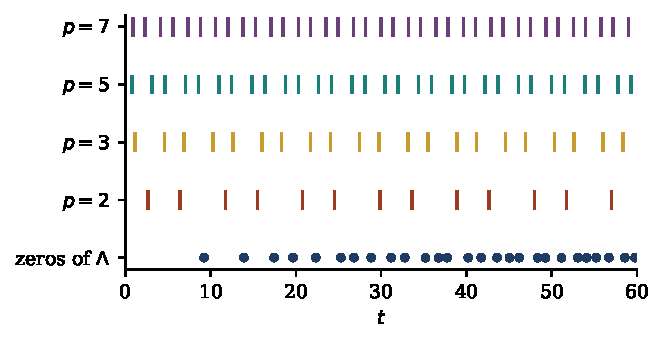
\includegraphics[width=\textwidth]{figs/thorin_combs.pdf}
\caption{Ordinates of the local zeros (local Thorin combs) of $\Delta$ at $p=2,3,5,7$, the progressions $(\pm\theta_p+2\pi\Z)/\log p$, against the ordinates $\gamma$ of the zeros of $\Lambda(s,\Delta)$ for $0<t<60$. Each comb is periodic with density $\log p/\pi$; the global zeros are not periodic.}\label{fig:10ccombs}
\end{figure}

\begin{remark}[Heuristic]
The combs of the primes $p\le P$ have total density $\sum_{p\le P}\log p/\pi\approx P/\pi$ by the prime number theorem, while the zeros of $L(s,\Delta)$ near height $t$ have density $\frac1\pi\log\frac{t}{2\pi}$. The two agree when $P\approx\log\frac{t}{2\pi}$: near height $t$, a truncated product of local GGCs over $p\lesssim\log t$ carries as many Thorin atoms per unit length as the global Thorin measure. This echoes the hybrid Euler Hadamard product $P_XZ_X$ of Gonek, Hughes and Keating \cite{ghk2007} (Section~\ref{sec:09bhybrid}), whose splitting conjecture is posed for $X=O((\log T)^{2-\varepsilon})$, a range that contains the matching scale $X\approx\log T$.
\end{remark}

The Euler product itself does not converge to a global GGC: the local means $(\log p)^2/(2-x_p)$ are not summable, and the global Thorin measure is not the sum of the local combs. The explicit formula, read through Proposition~\ref{prop:10cdictionary}, is the precise relation between them.

\section{Sato Tate random Euler products}\index{Thorin point process}

Model the angles $\theta_p$ as independent random variables with the Sato Tate law $\frac2\pi\sin^2\theta\,d\theta$ on $[0,\pi]$. By Theorem~\ref{thm:10clocal} every local reciprocal factor $f_{x_p}$, $x_p=2\cos\theta_p$, is the Laplace transform of a GGC almost surely (the only excluded value, $\theta_p=0$, has probability zero), and for every $P$ the truncated random Euler product
\[
\Phi_P(s)=\prod_{p\le P}\frac{2-x_p}{2\cosh(\sqrt s\log p)-x_p}
\]
is the Laplace transform of a GGC whose Thorin measure $\tau_P=\sum_{p\le P}\tau_{\theta_p,\log p}$ is random. We call $\tau_P$, or its preimage on the ordinate axis, a \emph{Thorin point process}.

\begin{proposition}[this book]\label{prop:10csatotate}
Let $\theta$ have the Sato Tate law and let $\epsilon=\pm1$ be an independent fair sign.
\begin{enumerate}
\item The configuration $\{\theta,-\theta\}$ on the circle $\R/2\pi\Z$ has intensity $\frac2\pi\sin^2\psi\,d\psi$, and $\epsilon\theta$ has density $\frac1\pi\sin^2\psi$ on $(-\pi,\pi]$.
\item The ordinates $(\pm\theta+2\pi\Z)/\log p$ of the comb of $p$ form a symmetric point process on $\R$ with intensity
\[
\frac{\log p}{\pi}\bigl(1-\cos(2t\log p)\bigr)\,dt .
\]
Consequently the Thorin point process of $\Phi_P$ has intensity $I_P(t)\,dt$ on the ordinate axis, $I_P(t)=\frac1\pi\sum_{p\le P}\log p\,(1-\cos(2t\log p))$.
\item $\E[(2-x_p)^{-1}]=1$, so the local law has expected mean $(\log p)^2$.
\end{enumerate}
\end{proposition}

\begin{proof}
(1) For a test function $\phi$ on the circle, $\E[\phi(\theta)+\phi(-\theta)]=\int_0^\pi(\phi(\psi)+\phi(-\psi))\frac2\pi\sin^2\psi\,d\psi=\int_{-\pi}^{\pi}\phi(\psi)\frac2\pi\sin^2\psi\,d\psi$, and half of this is $\E\phi(\epsilon\theta)$.

(2) Let $L=\log p$ and $\phi$ be compactly supported on $\R$. By (1) and unfolding the sum over $k$,
\begin{align*}
\E\sum_{k\in\Z}\Bigl[\phi\Bigl(\frac{\theta+2\pi k}{L}\Bigr)+\phi\Bigl(\frac{-\theta+2\pi k}{L}\Bigr)\Bigr]&=\sum_k\int_{-\pi}^{\pi}\phi\Bigl(\frac{\psi+2\pi k}{L}\Bigr)\frac2\pi\sin^2\psi\,d\psi\\
&=\int_{\R}\phi\Bigl(\frac uL\Bigr)\frac2\pi\sin^2u\,du,
\end{align*}
using periodicity of $\sin^2$. Substituting $u=Lt$ and $2\sin^2(Lt)=1-\cos(2Lt)$ gives the intensity. Intensities of independent superpositions add.

(3) With $x=2\cos\theta$, $2-x=4\sin^2(\theta/2)$ and $\sin^2\theta=4\sin^2(\theta/2)\cos^2(\theta/2)$, so $\E(2-x)^{-1}=\frac2\pi\int_0^\pi\cos^2(\theta/2)\,d\theta=1$. The mean of the local law is $L^2/(2-x)$ by Theorem~\ref{thm:10clocal}.
\end{proof}

Compare two other models. If $\theta_p$ is uniform on $[0,\pi]$ (the arcsine law for $x_p$), the comb of $p$ has flat intensity $\log p/\pi$. Under the law $\mu_{\mathrm{CM}}=\frac12\delta_0+\frac12\,$arcsine of Chapter~\ref{ch:04}, half the primes have $\theta_p=\pi/2$ and contribute the deterministic comb $(\frac12+\Z)\pi/\log p$, the other half the flat intensity, so the intensity is $\frac{\log p}{2\pi}+\frac12\sum_{k\in\Z}\delta_{(k+1/2)\pi/\log p}$. Only the Sato Tate model depletes the origin: $I_P(0)=0$ and $I_P(t)\le\frac{2t^2}{\pi}\sum_{p\le P}(\log p)^3$, a quadratic vanishing at $t=0$ (and at no other point once two primes are present). Part (3) shows the same effect in the mean: under the arcsine model $\E(2-x_p)^{-1}=\infty$, because angles near $0$ put Thorin atoms near the origin, while under Sato Tate the depletion makes the expected mean finite.

We read this cautiously. Of the one level densities of Section~\ref{sec:ch6ks}, $W(\USp)$ vanishes quadratically at the central point, and so does $W(\mathrm{SO(odd)})$ once the forced central zero is removed, while $W(\mathrm{SO(even)})$ does not \cite{ils2000,katzsarnak1999}. The Sato Tate depletion near $t=0$ is a local mechanism with the sign and the order of vanishing of the symplectic case, built prime by prime from the factor $\sin^2$ in the Haar measure of $\SU(2)=\USp(2)$. At the scale $t\asymp1/\log P$ the prime number theorem gives $I_P(t)=\frac1\pi\bigl(\vartheta(P)-\Re\frac{P^{1+2it}}{1+2it}\bigr)+o(P)$, with $\vartheta$ Chebyshev's function, so the depletion has width of order $1/\log P$. We do not claim that the global one level density is a consequence of this local picture; the heuristic of the previous section suggests matching $\log P$ with $\log\log t$, and making any such statement precise is open.

\section[Function fields and graphs: unconditional global Thorin]{Function fields and graphs:\\ unconditional global Thorin}\index{function field}

Let $C$ be a smooth projective geometrically connected curve of genus $g\ge1$ over $\mathbb F_q$. Its zeta function is
\[
Z(C,u)=\frac{P(u)}{(1-u)(1-qu)},\qquad P(u)=\prod_{j=1}^{2g}(1-\alpha_ju)\in\Z[u],\qquad u=q^{-s},
\]
and the functional equation makes the multiset $\{\alpha_j\}$ stable under $\alpha\mapsto q/\alpha$. Pair the roots accordingly, and for each pair put $c_j=(\alpha_j+q/\alpha_j)/\sqrt q$, $1\le j\le g$. With $z=s-\frac12$ and $u=q^{-1/2-z}$, each pair gives $(1-\alpha_ju)(1-(q/\alpha_j)u)=q^{-z}\bigl(2\cosh(z\log q)-c_j\bigr)$, so
\[
\Xi_C(z):=q^{gz}P(q^{-1/2-z})=\prod_{j=1}^g\bigl(2\cosh(z\log q)-c_j\bigr),
\]
an even entire function, real on the real axis. The Riemann hypothesis for $C$ is $|\alpha_j|=\sqrt q$ for all $j$, equivalently $c_j=2\cos\theta_j\in[-2,2]$ with $\alpha_j=\sqrt q\,e^{i\theta_j}$. It was proved by Weil \cite{weil1948}, and in all dimensions by Deligne \cite{deligne1974}. Put $F_C(s)=\Xi_C(\sqrt s)/\Xi_C(0)$.

\begin{theorem}[this book]\label{thm:10ccurve}
Assume $P(q^{-1/2})\ne0$, that is, no $\alpha_j$ equals $\sqrt q$. Then $s\mapsto1/F_C(s)$ is the Laplace transform of a GGC if and only if the Riemann hypothesis holds for $C$. In that case the Thorin measure is the finite superposition of periodic combs
\[
\tau_C=\sum_{j=1}^g\sum_{k\in\Z}\delta_{((\theta_j+2\pi k)/\log q)^2},
\]
and the law is $\sum_j\sum_kE_{j,k}\,(\log q)^2/(\theta_j+2\pi k)^2$, with mean $(\log q)^2\sum_j(2-c_j)^{-1}$. By Weil's theorem all of this holds unconditionally.
\end{theorem}

\begin{proof}
If the Riemann hypothesis holds then every $c_j\in[-2,2)$, the value $2$ being excluded by $P(q^{-1/2})\ne0$, and $1/F_C=\prod_jf_{c_j}$ with $L=\log q$. Each factor is a GGC transform with Thorin measure $\tau_{\theta_j,\log q}$ by Theorem~\ref{thm:10clocal}, and GGCs are closed under convolution, Thorin measures adding. Conversely, suppose $1/F_C$ agrees on $(0,\infty)$ with the Laplace transform $\varphi$ of a GGC. By Lemma~\ref{lem:ch10nonvanish}, $\varphi F_C$ is holomorphic on $\C\setminus(-\infty,0]$, and it equals $1$ on $(0,\infty)$, hence everywhere; so the entire function $s\mapsto\Xi_C(\sqrt s)$ has no zeros off $(-\infty,0]$, and since $\Xi_C(0)\ne0$ every zero $z$ of $\Xi_C$ is purely imaginary. A zero of $2\cosh(z\log q)-c_j$ with $z=iy$ satisfies $\cos(y\log q)=c_j/2$, which forces $c_j\in[-2,2]$. Hence every $c_j$ is real in $[-2,2]$ and $|\alpha_j|=\sqrt q$.
\end{proof}

\begin{example}
For $C:y^2=x^5-x+1$ over $\mathbb F_{101}$ (genus $2$) the characteristic polynomial of Frobenius, computed for this book, is $T^4+8T^3-16T^2+808T+10201$, so $\#C(\mathbb F_{101})=110$. All roots have absolute value $\sqrt{101}$, with angles $\theta_1=0.973934$, $\theta_2=2.858029$, so $c_1=1.124099$, $c_2=-1.920129$ and $\Xi_C(0)=P(101^{-1/2})=3.433644$. The smallest Thorin atoms are $0.044534$, $0.383502$, $0.550801$, $1.323428$, and the GGC has mean $29.7504$. The product identity of Lemma~\ref{lem:10cproduct} at these angles, truncated at $|k|\le20000$, was checked to relative error $1.3\times10^{-5}$.
\end{example}

The same holds for regular graphs. Let $G$ be a finite connected $(q+1)$ regular graph with adjacency eigenvalues $\lambda_j$. By the Ihara Bass formula of Chapter~\ref{ch:08}, each eigenvalue contributes $1-\lambda_ju+qu^2=q^{-z}(2\cosh(z\log q)-\lambda_j/\sqrt q)$ at $u=q^{-1/2-z}$. The trivial eigenvalue $q+1$ gives $x=\sqrt q+1/\sqrt q>2$, which in Theorem~\ref{thm:10clocal} is a positive real pole: it plays the role of the pole of $\zeta$ at $s=1$, and the Thorin criterion rejects it, as the global criterion must reject the pole. Put
\[
\Xi_G(z)=\prod_{|\lambda_j|<q+1}\Bigl(2\cosh(z\log q)-\frac{\lambda_j}{\sqrt q}\Bigr),\qquad F_G(s)=\frac{\Xi_G(\sqrt s)}{\Xi_G(0)} .
\]

\begin{theorem}[this book]\label{thm:10cihara}\index{Ramanujan graph}
Suppose no eigenvalue of $G$ equals $2\sqrt q$. Then $G$ is Ramanujan if and only if $1/F_G$ is the Laplace transform of a GGC, and then its Thorin measure is $\sum_j\sum_{k\in\Z}\delta_{((\theta_j+2\pi k)/\log q)^2}$ over the nontrivial eigenvalues $\lambda_j=2\sqrt q\cos\theta_j$. For the supersingular $\ell$ isogeny graphs $G_N(\ell)$ of Chapter~\ref{ch:08}, with $N\equiv1\bmod12$ and $\ell\ne N$ primes, both hold unconditionally.
\end{theorem}

\begin{proof}
The first statement is the proof of Theorem~\ref{thm:10ccurve} with $c_j=\lambda_j/\sqrt q$. For $G_N(\ell)$, Theorem~\ref{thm:08brandt} identifies the nontrivial spectrum with the eigenvalues of $T_\ell$ on $S_2(\Gamma_0(N))$, which satisfy $|\lambda|\le2\sqrt\ell$. The eigenvalue $2\sqrt\ell$ does not occur: $\lambda=\pm2\sqrt\ell$ would mean equal Satake parameters, excluded in weight two by Coleman and Edixhoven \cite{colemanedixhoven1998}.
\end{proof}

The shape of the Thorin measures separates function fields from $\Q$. Over a function field the global Thorin measure is a finite superposition of $g$ periodic combs with common period $2\pi/\log q$ on the ordinate axis, because $\Xi_C$ is a polynomial in $\cosh(z\log q)$. Over $\Q$ the ordinates that carry the global Thorin measure of Chapter~\ref{ch:10b} are aperiodic, with density growing like $\log t$, and the explicit formula, read through Proposition~\ref{prop:10cdictionary}, shows them as the interference pattern of infinitely many local combs, each damped by its half shift, whose base frequencies $\log p$ are linearly independent over $\Q$ by unique factorisation. Ramanujan is local Thorin in both worlds; global Thorin is known only where there is one comb period.

\section{Hecke walks and Thorin measures of passage times}\index{Keilson's theorem}\index{passage time}

In this section the Thorin measures are spectra. Let $Y$ be a birth death process on $\{0,1,\dots,n\}$ with birth rates $b_k>0$ ($0\le k<n$) and death rates $d_k>0$ ($1\le k\le n$), reflecting at $0$, started at $0$, and let $T$ be its first passage time to $n$. Let $Q_n$ be the generator restricted to $\{0,\dots,n-1\}$ (killed at $n$).

\begin{theorem}[Keilson \cite{keilson1971}]\label{thm:10ckeilson}
The eigenvalues $\lambda_1<\dots<\lambda_n$ of $-Q_n$ are real, simple and positive, and $T$ has the law of $\sum_{j=1}^nE_j/\lambda_j$. In particular $T$ is a GGC with Thorin measure $\sum_j\delta_{\lambda_j}$, and $\E e^{-sT}=\det(-Q_n)/\det(sI-Q_n)$.
\end{theorem}

\begin{proof}
For $s>0$ let $u_k=\E_ke^{-sT}$, $0\le k<n$. First step analysis gives $(sI-Q_n)u=b_{n-1}e_{n-1}$. By Cramer's rule $u_0$ is $b_{n-1}$ times the $(n-1,0)$ cofactor of $sI-Q_n$, divided by $\det(sI-Q_n)$. Deleting row $n-1$ and column $0$ of the tridiagonal matrix $sI-Q_n$ leaves a triangular matrix with diagonal $-b_0,\dots,-b_{n-2}$, so the cofactor equals $b_0\cdots b_{n-2}$, independent of $s$. Hence $u_0=b_0\cdots b_{n-1}/\det(sI-Q_n)$, and letting $s\to0$, where $u_0\to\Prob_0(T<\infty)=1$, gives $\det(-Q_n)=b_0\cdots b_{n-1}\ne0$. The matrix $-Q_n$ is similar, by the diagonal matrix of square roots of the reversible weights, to a symmetric Jacobi matrix with nonzero off diagonal entries $-\sqrt{b_kd_{k+1}}$; so its eigenvalues are real and simple. Each row of $-Q_n$ has diagonal entry at least the sum of the moduli of its off diagonal entries, so by Gershgorin's theorem the eigenvalues are nonnegative, and since $\det(-Q_n)\ne0$ they are positive. Therefore $\E e^{-sT}=\prod_j\lambda_j/(s+\lambda_j)$, the Laplace transform of $\sum_jE_j/\lambda_j$.
\end{proof}

Kent proved the analogue for one dimensional diffusions, with infinitely many rates \cite{kent1980}, and Fill gave a probabilistic proof by a stochastic construction of the exponential stages \cite{fill2009}. An exercise of Chapter~\ref{ch:10} uses the hitting time of a Bessel process in the same way.

Let $\T_q$ be the $(q+1)$ regular tree, the Bruhat Tits tree of $\PGL_2(\Q_q)$ for $q$ prime, and run continuous time simple random walk on it, jumping at rate $1$ to a uniformly chosen neighbour; this is the Hecke walk with generator $(q+1)^{-1}A-I$, where $A=T_q$ is the adjacency operator of Chapter~\ref{ch:07}. Let $T_n$ be the first time at distance $n$ from the start. The distance is a birth death process with $b_0=1$, and $b_k=\frac{q}{q+1}$, $d_k=\frac1{q+1}$ for $k\ge1$. Symmetrising,
\[
-Q_n\sim J_n=I-S_n,\qquad S_n=\begin{pmatrix}0&a&&&\\a&0&c&&\\&c&0&\ddots&\\&&\ddots&\ddots&c\\&&&c&0\end{pmatrix},
\]
with $a=1/\sqrt{q+1}$ and $c=\sqrt q/(q+1)=\rho/2$, where $\rho=2\sqrt q/(q+1)$ is the Kesten spectral radius.

\begin{theorem}[Passage times on the tree, this book]\label{thm:10ctree}\index{Kesten band}
Let $q\ge2$, $\rho=2\sqrt q/(q+1)$, and let $\lambda_1<\dots<\lambda_n$ be the Thorin atoms of $T_n$.
\begin{enumerate}
\item $\lambda_j=1-\frac{\sqrt q}{q+1}x_j$, where $x_1>\dots>x_n$ are the zeros of the polynomial $U_n(x/2)-q^{-1}U_{n-2}(x/2)$ that expresses $B_n=q^{-n/2}A_n$ in terms of $X=q^{-1/2}A$ (Theorem~\ref{thm:07tree}). All $x_j$ lie in $(-2,2)$, so all rates lie in the Kesten band $(1-\rho,1+\rho)$.
\item $\frac1n\sum_j\delta_{\lambda_j}$ converges weakly to the law of $1-\rho\cos(\pi U)$, $U$ uniform on $(0,1)$: the arcsine law on the Kesten band.
\item $\E T_n=\frac{n(q+1)}{q-1}-\frac{2q(1-q^{-n})}{(q-1)^2}$, and $\E T_n/n\to\frac{q+1}{q-1}=\frac1{\sqrt{1-\rho^2}}=\int_0^1\frac{du}{1-\rho\cos\pi u}$. The escape speed of the walk is $\frac{q-1}{q+1}=\sqrt{1-\rho^2}$.
\item $\mathrm{Var}\,T_n/n\to\bigl(\frac{q+1}{q-1}\bigr)^3=(1-\rho^2)^{-3/2}$, and $(T_n-\E T_n)/\sqrt{\mathrm{Var}\,T_n}$ converges in law to a standard normal.
\end{enumerate}
\end{theorem}

\begin{proof}
(1) Let $D_k$ be the characteristic polynomial of the leading $k\times k$ block of $c^{-1}S_n$, whose first off diagonal entry is $a/c=\sqrt{1+1/q}$ and the others $1$. Expanding along the last row, $D_1=x$, $D_2=x^2-1-q^{-1}$ and $D_{k+1}=xD_k-D_{k-1}$ for $k\ge2$. The polynomials $U_k(x/2)-q^{-1}U_{k-2}(x/2)$, with $U_{-1}=0$, satisfy the same recursion for $k\ge2$ and agree with $D_1$, $D_2$ and $D_3=x^3-(2+q^{-1})x$ at $k=1,2,3$, so they equal $D_k$; by Theorem~\ref{thm:07tree}(1) this is the polynomial of $B_k$. The eigenvalues of $S_n$ are $cx_j$, so $\lambda_j=1-cx_j$. To locate the zeros put $x=2\cos\phi$, $0<\phi<\pi$; then $D_n=g(\phi)/\sin\phi$ with
\[
g(\phi)=\sin((n+1)\phi)-q^{-1}\sin((n-1)\phi).
\]
At $\phi_k^*=(k+\frac12)\pi/(n+1)$, $0\le k\le n$, $|\sin((n+1)\phi)|=1>q^{-1}$, so $g(\phi_k^*)$ has the sign $(-1)^k$. Hence $g$ has a zero $\phi_j$ in each interval $(\phi_{j-1}^*,\phi_j^*)$, $1\le j\le n$. These are $n$ distinct zeros in $(0,\pi)$, and $D_n$ has degree $n$, so they are all the zeros and $x_j=2\cos\phi_j\in(-2,2)$. Since $c\cdot2=\rho$, $\lambda_j=1-\rho\cos\phi_j\in(1-\rho,1+\rho)$.

Conceptually, $S_n$ is a compression of the radial part of $P=(q+1)^{-1}A$, whose spectrum lies in $[-\rho,\rho]$ by Kesten's theorem~\cite{kesten1959}, so the rates cannot leave the closed Kesten band.

(2) The bracketing $\phi_j\in(\phi_{j-1}^*,\phi_j^*)$ gives $|\phi_j-j\pi/(n+1)|<\pi/(2(n+1))$, so for continuous $\psi$ on $[1-\rho,1+\rho]$, $\frac1n\sum_j\psi(1-\rho\cos\phi_j)$ is a Riemann sum converging to $\int_0^1\psi(1-\rho\cos\pi u)\,du$. It also follows from Szeg\H{o}'s theorem for Toeplitz matrices \cite{grenandersz}, since $S_n$ differs from the tridiagonal Toeplitz matrix with symbol $\rho\cos\phi$ by a perturbation of rank two, and by interlacing such a perturbation moves the empirical spectral measure by at most $2/n$ in Kolmogorov distance.

(3) Let $m_k$ be the expected time to go from distance $k$ to $k+1$. Then $m_0=1$, and for $k\ge1$ the walk waits a mean unit time and then moves down with probability $\frac1{q+1}$, after which it needs $m_{k-1}+m_k$ more on average: $m_k=1+\frac{1}{q+1}(m_{k-1}+m_k)$, that is $m_k=\frac{q+1}{q}+\frac{m_{k-1}}{q}$. With $m^*=\frac{q+1}{q-1}$ this is $m_k-m^*=(m_{k-1}-m^*)/q$, so $m_k=m^*-\frac{2}{q-1}q^{-k}$, and summing $k=0,\dots,n-1$ gives the formula. The limit of $\E T_n/n=\frac1n\sum_j\lambda_j^{-1}$ also follows from (2), since $1/\lambda$ is continuous on the band, together with $\int_0^\pi\frac{d\phi}{\pi(1-\rho\cos\phi)}=(1-\rho^2)^{-1/2}$ and $1-\rho^2=\bigl(\frac{q-1}{q+1}\bigr)^2$. For the speed, away from $0$ the distance jumps at rate $1$, up with probability $\frac q{q+1}$ and down with probability $\frac1{q+1}$, and it visits $0$ only finitely often, so by the law of large numbers the distance at time $t$ divided by $t$ tends almost surely to $\frac{q-1}{q+1}=1/m^*$.

(4) $\mathrm{Var}\,T_n=\sum_j\lambda_j^{-2}$, and (2) with $\int_0^\pi\frac{d\phi}{\pi(1-\rho\cos\phi)^2}=(1-\rho^2)^{-3/2}$ gives the limit. The summands $E_j/\lambda_j$ are independent with $\E|E_j-1|^3\lambda_j^{-3}\le C(1-\rho)^{-3}$, so the Lyapunov ratio is $O(n(1-\rho)^{-3}/n^{3/2})\to0$.
\end{proof}

Thus the Thorin rates of the passage time are $1-\frac{\sqrt q}{q+1}x$ with $x$ in the tempered spectrum $[-2,2]$: the statement \emph{Thorin support in the Kesten band} is the random walk form of the Ramanujan bound. Kesten's spectral radius determines the escape speed through the arcsine average of the reciprocal rates; in Chapter~\ref{ch:07} the same number is the drift $\frac{q-1}{q+1}$ of the distance chain, whose gambler's ruin gives the return probability $1/q$.

The theorem also gives exact large deviations. Since all rates exceed $1-\rho$, $\E e^{\theta T_n}=\prod_j(1-\theta/\lambda_j)^{-1}$ is finite for $\theta\le1-\rho$, and we can compute the limit through the Thorin measure.

\begin{theorem}[Large deviations of passage times, this book]\label{thm:10cldp}
For $\theta\le1-\rho$,
\[
\lim_{n\to\infty}\frac1n\log\E e^{\theta T_n}=\Lambda(\theta)=-\log\frac{(q+1)\bigl(1-\theta+\sqrt{(1-\theta)^2-\rho^2}\bigr)}{2q},
\]
and the limit is $+\infty$ for $\theta>1-\rho$. In particular $\Lambda(1-\rho)=\frac12\log q$. The function $\Lambda$ is steep, $\Lambda'(\theta)=((1-\theta)^2-\rho^2)^{-1/2}\to\infty$ as $\theta\uparrow1-\rho$, so $T_n/n$ satisfies a large deviation principle with good rate function
\[
\Lambda^*(y)=y-\sqrt{1+\rho^2y^2}+\log\frac{(q+1)\bigl(1+\sqrt{1+\rho^2y^2}\bigr)}{2qy},\qquad y>0,
\]
which vanishes only at $y=\frac{q+1}{q-1}$.
\end{theorem}

\begin{proof}
For $\theta<1-\rho$, $\frac1n\log\E e^{\theta T_n}=\frac1n\sum_j\bigl[\log\lambda_j-\log(\lambda_j-\theta)\bigr]$, and the integrand is continuous on the band, so by Theorem~\ref{thm:10ctree}(2) the limit is $\int_0^\pi[\log(1-\rho\cos\phi)-\log(1-\theta-\rho\cos\phi)]\frac{d\phi}{\pi}$. The classical integral $\int_0^\pi\log(a-b\cos\phi)\frac{d\phi}\pi=\log\frac{a+\sqrt{a^2-b^2}}{2}$ for $a\ge|b|$, together with $1+\sqrt{1-\rho^2}=\frac{2q}{q+1}$, gives $\Lambda$. At $\theta=1-\rho$ the second term becomes $\log(\rho(1-\cos\phi))$, which is singular at $\phi=0$, but it is increasing in $\phi$ and integrable, and the bracketing of the $\phi_j$ in intervals of length $\pi/(n+1)$ shows that its Riemann sums converge to the integral (the term $j=1$ is $O(n^{-1}\log n)$). The value is $-\log\frac{(q+1)\rho}{2q}=\frac12\log q$. For $\theta>1-\rho$, $\lambda_1\to1-\rho$ by (2), so $\E e^{\theta T_n}=\infty$ for large $n$. Differentiating, $\Lambda'(\theta)=((1-\theta)^2-\rho^2)^{-1/2}$, which tends to infinity at the edge, so $\Lambda$ is essentially smooth with $0$ in the interior of its domain and the G\"artner Ellis theorem \cite{dembozeitouni1998} applies. Since $\Lambda'$ maps $(-\infty,1-\rho)$ onto $(0,\infty)$, the supremum in $\Lambda^*(y)=\sup_\theta[\theta y-\Lambda(\theta)]$ is attained at $1-\theta=\sqrt{\rho^2+y^{-2}}$, and substituting gives the formula. At $y=(1-\rho^2)^{-1/2}$ one finds $\sqrt{1+\rho^2y^2}=y$ and $\Lambda^*(y)=0$.
\end{proof}

The value $\Lambda(1-\rho)=\frac12\log q$ is half the logarithm of the branching number: at the edge of the Kesten band the exponential moment grows like $q^{n/2}$, and indeed the closed form $\E e^{(1-\rho)T_n}=\frac{q+1}{q}\,q^{n/2}\big/\bigl(n+1-\frac{n-1}{q}\bigr)$, which follows from Theorem~\ref{thm:10ckeilson} and the values of $D_n$ at $x=2$ and $x=1/c$, shows the polynomial correction. For $q=2$ and $n=6400$ it gives $\frac1n\log\E e^{(1-\rho)T_n}=0.345376$, the value computed from the rates, against the limit $\frac12\log2=0.346574$.

The numbers, computed for this book from the Jacobi matrices $J_n$ for $q=2,3,5$ and $n=100,400,1600,6400$, confirm every statement. All rates lie in $(1-\rho,1+\rho)$; at $n=6400$ the smallest rates are $0.05719$, $0.13397$, $0.25464$ against gaps $1-\rho=0.057191$, $0.133975$, $0.254644$. The ratios $\E T_n/n$ are $2.99938$, $1.99977$, $1.49990$ against $3$, $2$, $1.5$, and $\mathrm{Var}\,T_n/n=26.9856$, $7.9975$, $3.3744$ against $27$, $8$, $3.375$. The trace $\mathrm{tr}\,J_n^{-1}=19196$ for $q=2$, $n=6400$ equals the formula of (3). The Kolmogorov distance of the rescaled rates to the arcsine law is $8\times10^{-5}$ at $n=6400$. For $q=2$ and $n=6400$, $\frac1n\log\E e^{\theta T_n}$ is $-0.693095$ at $\theta=-0.5$ against $\Lambda=-0.693147$, and $0.100872$ at $\theta=(1-\rho)/2=0.0286$ against $0.100899$. A simulation of $20000$ walks with $q=2$, $n=100$ gave mean $296.07$, against $296.24$ for an equal sample from $\sum E_j/\lambda_j$ and the exact value $296$; the Kolmogorov Smirnov test comparing the two samples has $p=0.57$ (Figure~\ref{fig:10ctree}).

\begin{figure}[t]\centering
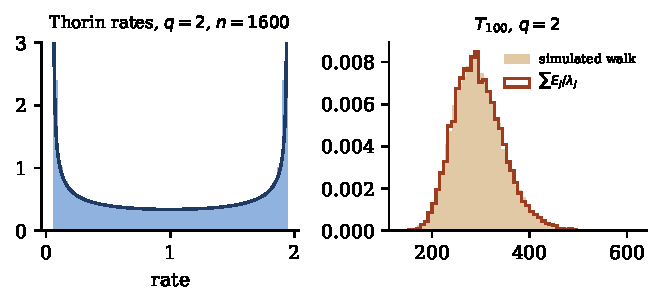
\includegraphics[width=\textwidth]{figs/thorin_tree.pdf}
\caption{Left: the Thorin atoms of $T_{1600}$ for $q=2$ against the arcsine density on the Kesten band $(1-\rho,1+\rho)$. Right: simulated passage times $T_{100}$ ($q=2$, $20000$ walks) against the GGC $\sum_jE_j/\lambda_j$ of Theorem~\ref{thm:10ckeilson}.}\label{fig:10ctree}
\end{figure}

\section{Exponential hitting times on Ramanujan graphs}\index{hitting time}\index{Aldous Brown inequality}

On a finite graph a passage time is no longer a pure GGC, but the spectral structure survives. Let $G$ be a connected $(q+1)$ regular graph with vertex set $V$ of size $h$ that is not bipartite. Loops and multiple edges are allowed, but the adjacency matrix $A$ is symmetric, as for the Brandt matrices of Chapter~\ref{ch:08} when $N\equiv1\bmod12$. Let $P=(q+1)^{-1}A$, with eigenvalues $1=p_1>p_2\ge\dots\ge p_h>-1$ (written $\mu_j$ in Appendix~\ref{app:A}; below, $\mu_j$ is a rate), and run the continuous time walk with generator $P-I$. Fix a target $v$ and let $\tau_v$ be its hitting time. Let $P_v$ be the principal submatrix of $P$ on $V\setminus\{v\}$, with eigenvalues $r_1\ge r_2\ge\dots\ge r_{h-1}$ and orthonormal eigenvectors $\psi_j$, and put $\mu_j=1-r_j$, the \emph{Dirichlet rates}.

\begin{proposition}\label{prop:10cmixture}
Started from the uniform law $\pi$,
\[
\Prob_\pi(\tau_v>t)=\sum_{j=1}^{h-1}w_je^{-\mu_jt},\qquad w_j=\frac1h\langle\vec 1,\psi_j\rangle^2\ge0,\qquad \sum_jw_j=\frac{h-1}{h},
\]
a completely monotone mixture of exponentials, and $\E_\pi\tau_v=\sum_jw_j/\mu_j\ge(h-1)^2/h$.
\end{proposition}

\begin{proof}
Killing at $v$, $\Prob_x(\tau_v>t)=(e^{-t(I-P_v)}\vec 1)(x)$ for $x\ne v$, and averaging over $x$ with weight $1/h$ gives the mixture by the spectral theorem for the symmetric matrix $P_v$. Connectedness makes $I-P_v$ positive definite. For the mean, $\E_\pi\tau_v=\frac1h\langle\vec 1,(I-P_v)^{-1}\vec 1\rangle$, and the Cauchy Schwarz inequality for the positive definite form gives $\langle\vec 1,M^{-1}\vec 1\rangle\langle\vec 1,M\vec 1\rangle\ge\langle\vec 1,\vec 1\rangle^2$ with $M=I-P_v$. Here $\langle\vec 1,\vec 1\rangle=h-1$, and since $P$ is symmetric and stochastic, $\langle\vec 1,M\vec 1\rangle=(h-1)-\sum_{x,y\ne v}P(x,y)=\sum_{x\ne v}P(x,v)=1-P(v,v)\le1$.
\end{proof}

The mixture form is classical (Keilson); see Aldous and Fill \cite{aldousfill}. By Cauchy interlacing the Dirichlet rates interlace the graph rates $1-p_j$, and these are what the Ramanujan bound controls.

\begin{theorem}[this book]\label{thm:10cexpo}
If $G$ is Ramanujan then $\mu_2,\dots,\mu_{h-1}\in[1-\rho,1+\rho]$, $\rho=2\sqrt q/(q+1)$: only the slowest Dirichlet rate $\mu_1\le1-p_2$ can leave the Kesten band. Moreover, for every target $v$,
\begin{align*}
\sup_{t\ge0}\bigl|\Prob_\pi(\tau_v>t)-e^{-t/\E_\pi\tau_v}\bigr|&\le\frac{\tau_2}{\E_\pi\tau_v}\le\frac{(q+1)\,h}{(\sqrt q-1)^2(h-1)^2}\\
&\le\frac{2(q+1)}{(\sqrt q-1)^2(h-1)},
\end{align*}
where $\tau_2=1/(1-p_2)$ is the relaxation time.
\end{theorem}

\begin{proof}
By Cauchy interlacing for the principal submatrix $P_v$ of the symmetric matrix $P$, $p_j\ge r_j\ge p_{j+1}$ for $1\le j\le h-1$. The Ramanujan property says $p_2,\dots,p_h\in[-\rho,\rho]$. For $j\ge2$, $r_j\le p_j\le p_2\le\rho$, and for all $j\le h-1$, $r_j\ge p_{j+1}\ge p_h\ge-\rho$. Hence $\mu_j=1-r_j\in[1-\rho,1+\rho]$ for $2\le j\le h-1$, and $\mu_1=1-r_1\le1-p_2$. The first inequality in the display is the Aldous Brown inequality for reversible chains started from stationarity \cite{aldousbrown1992,aldousfill}. Ramanujan gives $1-p_2\ge1-\rho=(\sqrt q-1)^2/(q+1)$, so $\tau_2\le(q+1)/(\sqrt q-1)^2$, and Proposition~\ref{prop:10cmixture} gives $\E_\pi\tau_v\ge(h-1)^2/h\ge(h-1)/2$.
\end{proof}

\begin{corollary}[Unconditional exponential law, this book]\label{cor:10cisogeny}
Let $N>13$ be a prime with $N\equiv1\bmod12$, so that $h=(N-1)/12\ge2$, and let $\ell\ne N$ be prime. For simple random walk in continuous time on the supersingular $\ell$ isogeny graph $G_N(\ell)$, every vertex $v$ satisfies
\[
\sup_{t\ge0}\bigl|\Prob_\pi(\tau_v>t)-e^{-t/\E_\pi\tau_v}\bigr|\le\frac{2(\ell+1)}{(\sqrt\ell-1)^2(h-1)},
\]
and all Dirichlet rates but the slowest lie in the Kesten band $[1-\rho_\ell,1+\rho_\ell]$, $\rho_\ell=2\sqrt\ell/(\ell+1)$.
\end{corollary}

\begin{proof}
By Theorem~\ref{thm:08brandt} every nontrivial eigenvalue satisfies $|\lambda|\le2\sqrt\ell<\ell+1$. Hence $\ell+1$ is a simple eigenvalue and $-(\ell+1)$ is not an eigenvalue, so $G_N(\ell)$ is connected, not bipartite and Ramanujan, and Theorem~\ref{thm:10cexpo} applies.
\end{proof}

Theorem~\ref{thm:08kemeny} supplies the scale. In continuous time at rate $1$ the expected hitting times are the discrete ones, so $\sum_v\pi(v)\E_\pi\tau_v$ is Kemeny's constant $K_N$, and $K_N/h\to\ell/(\ell-1)$. So on large isogeny graphs the time to find a given curve from a random start is, uniformly in time and up to $O(1/h)$, exponential, with a mean that averages over targets to about $\frac{\ell}{\ell-1}h$, that is about $2h$ for $\ell=2$.

The data, computed for this book on the supersingular $2$ isogeny graphs at $N=1009$, $2017$, $4129$, $7993$ ($h=84$, $168$, $344$, $666$) with six random targets each, are as follows. The largest observed $\sup_t|\Prob_\pi(\tau_v>t)-e^{-t/\E_\pi\tau_v}|$ is $0.0248$, $0.0144$, $0.0075$, $0.0039$; the Aldous Brown bound $\tau_2/\E_\pi\tau_v$ is $0.081$, $0.045$, $0.023$, $0.0127$; the Ramanujan bound of Corollary~\ref{cor:10cisogeny} is $0.421$, $0.209$, $0.102$, $0.0526$. The spectral gaps $1-p_2$ are $0.0845$, $0.0708$, $0.0642$, $0.0601$, above the Ramanujan lower bound $1-\rho_2=0.0572$; the smallest second Dirichlet rates are $\mu_2=0.0862$, $0.0710$, $0.0642$, $0.0601\ge0.0572$, and the largest Dirichlet rate is at most $1.9406\le1+\rho_2=1.9428$. All three quantities decay like $1/h$ (Figure~\ref{fig:10cisogeny}); the observed error is about a third of the Aldous Brown bound.

\begin{figure}[t]\centering
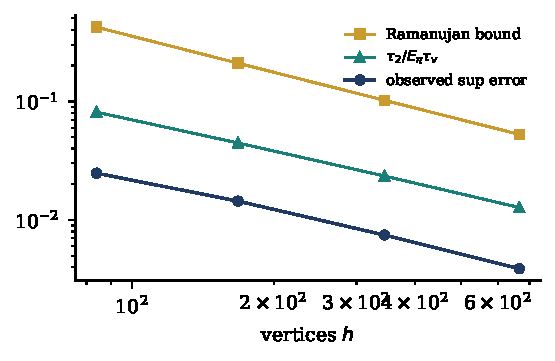
\includegraphics[width=0.8\textwidth]{figs/thorin_isogeny.pdf}
\caption{Supersingular $2$ isogeny graphs for $N=1009$, $2017$, $4129$, $7993$ ($h=84$ to $666$ vertices), six random targets $v$ each, logarithmic axes: the largest observed sup distance between $\Prob_\pi(\tau_v>t)$ and the exponential law with the same mean, against the largest Aldous Brown bound $\tau_2/\E_\pi\tau_v$ and the unconditional Ramanujan bound of Corollary~\ref{cor:10cisogeny}.}\label{fig:10cisogeny}
\end{figure}

\section{Extreme values and exponent measures}\index{max infinitely divisible}

Chapter~\ref{ch:11} represents $\prod_n(1-e^{-2\pi ny})$ as the distribution function of $M=\max_nE_n/(2\pi n)$. Here we identify the structure of $M$ in the language of this chapter: just as a GGC has a completely monotone L\'evy density, $M$ has a completely monotone exponent function. Write $\sigma_{-1}(m)=\sum_{d\mid m}d^{-1}$ and $P(y)=\Prob(M\le y)$ as in Chapter~\ref{ch:11}.

\begin{proposition}[this book]\label{prop:10cmaxid}
\begin{enumerate}
\item Let $G=-\log P$. Then for $y>0$
\[
G(y)=\sum_{m\ge1}\sigma_{-1}(m)\,e^{-2\pi my}.
\]
Hence $G$ is completely monotone, $G(y)=\int e^{-yu}\nu(du)$ with
\[
\nu=\sum_{m\ge1}\sigma_{-1}(m)\,\delta_{2\pi m},
\]
and $M$ is max infinitely divisible.
\item For each $n$, $E_n/(2\pi n)$ has the law of $\max_{k\ge1}\max_{i\le N_k}E_{k,i}/(2\pi nk)$, with $N_k$ Poisson of mean $1/k$, all variables independent. Consequently $M$ has the law of $\max_{m\ge1}\max_{i\le N'_m}E'_{m,i}/(2\pi m)$ with independent $N'_m$ Poisson of mean $\sigma_{-1}(m)$.
\item For $\Re s>1$, $\int_0^\infty G(y)y^{s-1}dy=\Gamma(s)(2\pi)^{-s}\zeta(s)\zeta(s+1)$. The right side continues meromorphically to $\C$ with poles only at $s=0,\pm1$, and is invariant under $s\mapsto-s$.
\item For $f=\prod_m\eta(m\tau)^{r_m}$ with $r_m\ge0$, $\sum_mmr_m=24$, and $M_f$ as in Theorem~\ref{thm:ch11general}, $-\log\Prob(M_f\le y)=\sum_mr_mG(my)$ is completely monotone with exponent measure $\sum_n\big(\sum_{m\mid n}r_m\sigma_{-1}(n/m)\big)\delta_{2\pi n}$, and its Mellin transform is $\Gamma(s)(2\pi)^{-s}\zeta(s)\zeta(s+1)\sum_mr_mm^{-s}$.
\end{enumerate}
\end{proposition}

\begin{proof}
(1) $-\log(1-e^{-2\pi ny})=\sum_{k\ge1}e^{-2\pi nky}/k$; summing over $n$ and collecting $m=nk$ gives $\sum_me^{-2\pi my}\sum_{k\mid m}k^{-1}$, and $\sum_{k\mid m}k^{-1}=\sigma_{-1}(m)$. A positive combination of decreasing exponentials is completely monotone. For every $t>0$, $P^t=\exp(-tG)$ is the distribution function of the maximum of a Poisson process with intensity $t\sum_m\sigma_{-1}(m)\,\mathrm{Law}(E/(2\pi m))$ by the computation in (2), so $M$ is max infinitely divisible \cite{resnick1987}.

(2) If $N$ is Poisson of mean $\lambda$, independent of the $Z_i$, independent copies of $Z$, then $\Prob(\max_{i\le N}Z_i\le y)=\E\Prob(Z\le y)^N=\exp(-\lambda\Prob(Z>y))$, with an empty maximum read as $0$. For $Z=E/(2\pi nk)$ and $\lambda=1/k$ this is $\exp(-e^{-2\pi nky}/k)$, and the product over $k$ is $\exp(\log(1-e^{-2\pi ny}))=1-e^{-2\pi ny}=\Prob(E_n/(2\pi n)\le y)$, by the identity $1-e^{-x}=\exp(-\sum_ke^{-kx}/k)$ for $x>0$. The maximum is almost surely over a nonempty set, since $\sum_k1/k=\infty$. Taking independent copies for all $n$ and merging the Poisson families with the same $m=nk$ (superposition adds the means $1/k$ over $k\mid m$) gives the second statement.

(3) By Tonelli's theorem the Mellin integral equals $\sum_m\sigma_{-1}(m)\Gamma(s)(2\pi m)^{-s}$, and $\sum_m\sigma_{-1}(m)m^{-s}=\sum_{d,k}d^{-s}k^{-1-s}=\zeta(s)\zeta(s+1)$ for real $s>1$, hence for $\Re s>1$. For the continuation use the modular relation~\eqref{eq:ch11Pmod}, which in terms of $G=-\log P$ reads $G(1/y)=G(y)-\frac12\log y-\frac{\pi}{12y}+\frac{\pi y}{12}$. Splitting the integral at $1$ and substituting $y\mapsto1/y$ on $(0,1)$,
\[
\int_0^\infty G(y)y^{s-1}dy=\int_1^\infty G(y)\bigl(y^{s-1}+y^{-s-1}\bigr)dy-\frac1{2s^2}-\frac{\pi}{12(s+1)}+\frac{\pi}{12(s-1)},
\]
using $\int_1^\infty y^{-s-1}\log y\,dy=s^{-2}$, $\int_1^\infty y^{-s-2}dy=(s+1)^{-1}$ and $\int_1^\infty y^{-s}dy=(s-1)^{-1}$. The integral is entire because $G$ decays exponentially, and it is invariant under $s\mapsto-s$, as are $-\frac1{2s^2}$ and the sum of the last two terms. Equivalently, the duplication formula gives $\Gamma(s)(2\pi)^{-s}\zeta(s)\zeta(s+1)=\frac12\hat\xi(s)\hat\xi(s+1)$ with $\hat\xi(s)=\pi^{-s/2}\Gamma(s/2)\zeta(s)$, and the symmetry is the functional equation $\hat\xi(s)=\hat\xi(1-s)$.

(4) $\Prob(M_f\le y)=\prod_mP(my)^{r_m}$ by definition, and (1) applied to each factor, with the Mellin substitution $y\mapsto my$, gives the rest.
\end{proof}

By (3), the exponent of the extreme value law of $\eta$ has Mellin transform $\Gamma(s)(2\pi)^{-s}\zeta(s)\zeta(s+1)$, a product of two shifted zeta functions of Eisenstein type, symmetric under $s\mapsto-s$, with a double pole at $s=0$ matching the term $\frac12\log y$ in the expansion of $G$ at $0$. Read backwards, Mellin inversion turns this symmetry into the modular relation, which is a classical proof of the transformation law of $\eta$; the probabilistic reading adds the exponent measure $\nu$ and the Poisson structure of (2). For every multiplicative eta product the exponent is Eisenstein, while the cusp form $L$ function enters only through the incomplete gamma expectation of Theorem~\ref{thm:ch11general}. The Poisson splitting identity in (2) is a max analogue of Frullani's integral: one exponential clock is a maximum over infinitely many Poisson families of faster clocks, just as one gamma variable is an integral of Poisson jumps.

\section{Notes}

The Thorin criterion for single Euler factors and its corollaries are ours; the ingredients are classical. Thorin \cite{thorin1977} and Bondesson \cite{bondesson1992} developed generalized gamma convolutions, and the Pringsheim Landau principle is in Widder's book \cite{widder1941}. Deligne \cite{deligne1974} proved the Ramanujan Petersson conjecture for holomorphic forms; for Maass forms the bound $\frac{7}{64}$ is due to Kim and Sarnak \cite{kimsarnak2003}, building on Kim and Shahidi \cite{kimshahidi2002}. Weil's explicit formula is in \cite{weil1952}, and our normalisation follows Iwaniec and Kowalski \cite{iwanieckowalski2004}. The hybrid product is from Gonek, Hughes and Keating \cite{ghk2007}, and one level densities from Iwaniec, Luo and Sarnak \cite{ils2000} and Katz and Sarnak \cite{katzsarnak1999}. Weil proved the Riemann hypothesis for curves in \cite{weil1948}; for graphs see Ihara \cite{ihara1966}, Lubotzky, Phillips and Sarnak \cite{lps1988} and Pizer \cite{pizer1990}. Keilson's theorem on passage times of birth death processes is \cite{keilson1971}, Kent's diffusion version \cite{kent1980}, and Fill's probabilistic proof \cite{fill2009}; the Aldous Brown inequality is \cite{aldousbrown1992}, and Aldous and Fill \cite{aldousfill} is the general reference for hitting times of reversible chains. Toeplitz spectra are in Grenander and Szeg\H{o} \cite{grenandersz}, large deviations in Dembo and Zeitouni \cite{dembozeitouni1998}, and max infinite divisibility in Resnick \cite{resnick1987}. The identification of passage time rates with zeros of the sphere polynomials $B_n$, the large deviation rate of Theorem~\ref{thm:10cldp}, the exponential law on isogeny graphs and the max infinitely divisible reading of Proposition~\ref{prop:10cmaxid} are, as far as we know, new; the Mellin transform in Proposition~\ref{prop:10cmaxid}(3) is classical.

\section{Exercises}

\begin{enumerate}
\item Comparing the coefficients of $w^4$ in Lemma~\ref{lem:10cproduct}, prove that
\[
\sum_{k\in\Z}\frac{1}{(\theta+2\pi k)^{4}}=\frac{2+\cos\theta}{48\sin^4(\theta/2)}.
\]
Deduce the variance of the local GGC of Theorem~\ref{thm:10clocal}, and show that under the Sato Tate law the expected variance is infinite.

\item\label{ex:10cdegenerate} Show that for $x_p=2$, $\frac{(\log p)^2s}{2\cosh(\sqrt s\log p)-2}=\prod_{k\ne0}\bigl(1+\frac{s(\log p)^2}{4\pi^2k^2}\bigr)^{-1}$, and interpret $1/E_p(\sqrt s)$ as a GGC with an extra degenerate Thorin atom of mass $1$ at the origin, as for a central zero of order two in Chapter~\ref{ch:10}.

\item Let $E$ be an elliptic curve over $\mathbb F_q$ with $a=q+1-\#E(\mathbb F_q)\ne2\sqrt q$. Show that the GGC of Theorem~\ref{thm:10ccurve} has mean $(\log q)^2\sqrt q/(\#E(\mathbb F_q)-(\sqrt q-1)^2)$, and that this mean is positive if and only if $\#E(\mathbb F_q)>(\sqrt q-1)^2$, one half of Hasse's bound $|a|\le2\sqrt q$. Show that the GGC property itself is equivalent to the full bound, and identify which half of it comes from the rejection of a real pole and which from Lemma~\ref{lem:10clandau}.

\item In Theorem~\ref{thm:10ctree} take $q=1$ (the reflecting walk on $\{0,1,2,\dots\}$, which is the line folded at the origin). Show that the rates are $1-\cos\frac{(2j-1)\pi}{2n}$, $1\le j\le n$, that $\E T_n=n^2$, and explain why the absence of a gap ($\rho=1$) turns the ballistic law of large numbers into diffusive scaling.

\item Derive the formula for $\Lambda^*$ in Theorem~\ref{thm:10cldp}, and show that $\Lambda^*(y)/y\to1-\rho$ as $y\to\infty$. Interpret: the probability of an atypically long passage time decays at the rate of the bottom of the Kesten band.

\item Using Proposition~\ref{prop:10cmaxid}(4), show that for $f=\eta(\tau)^2\eta(11\tau)^2$ the exponent function $-\log\Prob(M_f\le y)$ has Mellin transform
\[
2(1+11^{-s})\,\Gamma(s)(2\pi)^{-s}\zeta(s)\zeta(s+1),
\]
and compute the expected number of points of the Poisson representation of Proposition~\ref{prop:10cmaxid}(2), applied to each factor of $M_f$, that exceed $y$.
\end{enumerate}

\section{Open computational problems}

\begin{compproblem}[Comb statistics against the zeros of $\Delta$]
Objective: compare the Thorin point process intensity $I_P(t)$ of Proposition~\ref{prop:10csatotate}, with the actual angles $\theta_p$ of $\tau(p)$, against the zeros of $L(s,\Delta)$. Data: all zeros with $0<\gamma\le10^5$ (about $2.8\times10^5$), and $\tau(p)$ for $p\le10^7$. Route: PARI/GP \texttt{lfunzeros} or \texttt{lcalc} for the zeros, \texttt{ramanujantau} for the coefficients, with the explicit formula of Theorem~\ref{thm:10cexplicit} for Gaussian test functions of widths from $0.1$ to $10$ as a certificate. Deliverable: the pair correlation of local comb points against that of the zeros as a function of $P$ and $t$, a test of the heuristic matching $P\approx\log(t/2\pi)$, and a table of the per prime ratios of explicit formula terms to comb terms against $-p^{-1/2}$. Why it matters: it measures quantitatively how the aperiodic global Thorin measure is assembled from periodic local combs.
\end{compproblem}

\begin{compproblem}[Large deviations on finite isogeny graphs]
Objective: compare the cumulant generating function of distance passage times on supersingular isogeny graphs with the tree formula $\Lambda(\theta)$ of Theorem~\ref{thm:10cldp}. Data: $G_N(\ell)$ for $\ell=2,3$ and primes $N\equiv1\bmod12$ up to $10^5$ ($h$ up to about $8000$), with passage times to distance $n$ up to the injectivity radius. Route: build the graphs from modular polynomials in PARI/GP as in Chapter~\ref{ch:08}; compute $\E e^{\theta T_n}$ exactly by solving the killed linear systems for $\theta$ on a grid. Deliverable: plots of $n^{-1}\log\E e^{\theta T_n}$ against $\Lambda(\theta)$, the value at $\theta=1-\rho$ against $\frac12\log\ell$, and the distance $n(N)$ at which the finite graph departs from the tree. Why it matters: the departure measures how far the Ramanujan graph is from its universal cover at the scale of large deviations, a finer statistic than the spectrum.
\end{compproblem}

\begin{compproblem}[Kim Sarnak versus Ramanujan through local parabolas]
Objective: test the local parabolic conditions $\Theta^{(p)}_\sigma$ for Maass forms. Data: Hecke eigenvalues of Maass cusp forms for $\SL_2(\Z)$ and $\Gamma_0(N)$ with small $N$ from the LMFDB \cite{lmfdb}, for all available forms and primes. Route: compute $x_p$ and the largest $|\Re w|$ among the zeros of $E_p$; record any $|x_p|>2$. Deliverable: the empirical distribution of $\max_p|\Re w|$ per form against the proven bound $\frac{7}{64}$, the Sato Tate fit of the $x_p$, and a statistical test of the hypothesis that all local combs are on the axis. Why it matters: Ramanujan for Maass forms is open, and the local Thorin form makes every unramified prime a separate test with a quantitative margin.
\end{compproblem}

\begin{compproblem}[Thorin combs of curves of genus three and four]
Objective: measure how the periodic Thorin combs of Theorem~\ref{thm:10ccurve} fill the line in families. Data: all curves of genus $3$ and $4$ over $\mathbb F_q$ for $q\le13$ (hyperelliptic and plane quartic models in genus $3$), with their $L$ polynomials. Route: point counting in Sage or Magma, or the tables of Sutherland and collaborators where available. Deliverable: histograms of the angles $\theta_j$ against the $\USp(2g)$ Weyl density (Katz Sarnak \cite{katzsarnak1999}), the distribution of the smallest Thorin atom $(\min_j\theta_j/\log q)^2$, and the low lying angle density near $0$ compared with the Sato Tate depletion of Proposition~\ref{prop:10csatotate}. Why it matters: function fields are, with regular graphs, the setting where global Thorin is a theorem, and the statistics of the smallest atoms are the finite field model of low lying zeros.
\end{compproblem}
